\chapter{Incentives}
\label{ch:incentives}

The verbalizer was trained to maximise one number, the reconstruction cosine. If wrong names cost it
nothing, training never had a reason to remove them. This chapter tests that directly.

\section{Edit Test}

I took explanations at distances 0 and 1 that name the true entity and also contain at least one wrong name
in the part describing the context. There are 1{,}352 of them; I sampled 1{,}000. For each I made two edited
copies and sent all three through the reconstructor.

\begin{itemize}
\item \textbf{Wrong names removed.} Every wrong same-type name is replaced by a neutral phrase such as
``another city''. The true name stays.
\item \textbf{True name removed.} The true name is replaced the same way. The wrong names stay. This is the
control: it shows what an edit of the same size costs when it removes real information.
\end{itemize}

Writing $z^{-W}$ for the copy with wrong names removed and $z^{-e}$ for the copy with the true name removed,
the quantities of interest are what each kind of name is worth to the score of Equation~\ref{eq:score}:
\begin{equation}
\Delta_{\text{wrong}} = s(h,z) - s(h,z^{-W}), \qquad \Delta_{\text{true}} = s(h,z) - s(h,z^{-e}).
\label{eq:delta}
\end{equation}
If $\Delta_{\text{wrong}} \le 0$, the objective in Equation~\ref{eq:objective} would already discourage wrong
names. If it is near zero or positive, it does not.

The edits worked as intended: afterwards no wrong name is detected in 99.8\% of the first copies, and the
true name is gone from 94.3\% of the second.

\section{Results}

\begin{table}[t]
\centering
\footnotesize
\setlength{\tabcolsep}{3.5pt}
\resizebox{\linewidth}{!}{\begin{tabular}{@{}crlllll@{}}
\toprule
\shortstack[l]{Tokens after\\entity} & $n$ & Original & \shortstack[l]{Wrong names\\removed} & \shortstack[l]{True name\\removed} & \shortstack[l]{Original beats\\``wrong\\removed''} & \shortstack[l]{Original beats\\``true\\removed''} \\
\midrule
0 & 567 & 0.897 {\scriptsize[0.892, 0.902]} & 0.894 {\scriptsize[0.889, 0.899]} & 0.686 {\scriptsize[0.676, 0.695]} & 67.5 {\scriptsize[63.0, 72.1]} & 100.0 {\scriptsize[100.0, 100.0]} \\
1 & 433 & 0.895 {\scriptsize[0.886, 0.903]} & 0.889 {\scriptsize[0.880, 0.897]} & 0.879 {\scriptsize[0.869, 0.887]} & 79.9 {\scriptsize[75.5, 84.2]} & 88.2 {\scriptsize[84.1, 92.0]} \\
0 and 1 & 1{,}000 & 0.896 {\scriptsize[0.890, 0.901]} & 0.892 {\scriptsize[0.886, 0.897]} & 0.769 {\scriptsize[0.759, 0.779]} & 72.9 {\scriptsize[69.6, 76.1]} & 94.9 {\scriptsize[93.1, 96.6]} \\
\bottomrule
\end{tabular}
}
\caption[Reconstruction cosine before and after editing names out]{Reconstruction cosine before and after
editing names out, and how often the original scores higher than each edit (\%). Natural text; 95\%
intervals over passages.}
\label{tab:edit}
\end{table}

\begin{figure}[t]
\centering
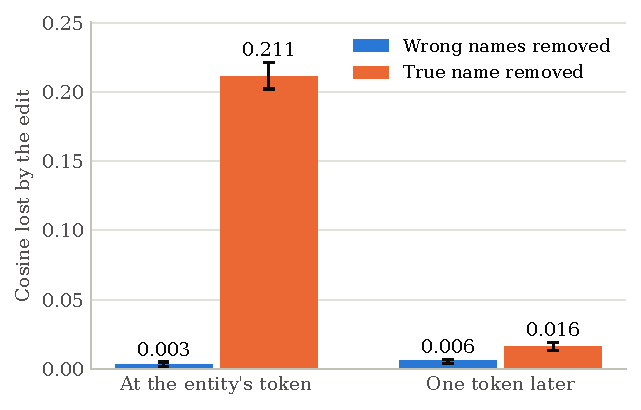
\includegraphics[width=0.6\linewidth]{edit}
\caption[What each kind of name is worth to the reconstruction score]{What each kind of name is worth to
the reconstruction score: cosine lost when it is edited out. Natural text; 95\% intervals.}
\label{fig:edit}
\end{figure}

$\Delta_{\text{wrong}}$ is 0.003 at the entity's token and 0.006 one token later (Table~\ref{tab:edit},
Figure~\ref{fig:edit}); per name removed, about 0.002. $\Delta_{\text{true}}$ is 0.211 at the entity's
token, seventy times as much, and 0.016 one token later.

\section{Interpretation}

Three things follow.

\textbf{Wrong names are nearly free, and slightly rewarded.} The original beats the cleaned copy 68\% of the
time at distance~0 and 80\% at distance~1. A wrong but plausible name of the right type reconstructs a
little better than a vague phrase, presumably because it still tells the reconstructor the type and the
topic. So the objective gives the verbalizer a small push towards naming \emph{something}.

\textbf{The true name stops mattering quickly.} It is worth 0.21 while the model is reading it and 0.016 a
single token later. From then on, getting the specific right earns almost nothing, so a verbalizer trained
only on reconstruction has little reason to keep track of it.

\textbf{This sets the scale for a fix.} A penalty of $\lambda$ per suspect name changes the reward to
$s(h,z) - \lambda\,|U(z)|$, where $U(z)$ is the set of names to discourage. For it to bite without also
driving out true names, $\lambda$ must sit between what a wrong name earns and what a true one earns:
\begin{equation}
0.002 \;\approx\; \Delta_{\text{wrong}} \text{ per name} \;<\; \lambda \;<\; \Delta_{\text{true}} \;\approx\; 0.016
\text{ (one token after the entity).}
\end{equation}
The fine-tuning experiments use $\lambda = 0.01$.

The verbalizer is doing what an autoencoder does: it keeps what helps reconstruction. The specific helps
very little, so nothing protects it.
